Poniższy rozdział omawia implementację aplikacji służącej jako intranet dla firmy z sektora IT, opisane zostaną założenia oraz --wymagania stawanie dla strony serwerowej oraz dla klientów--. W rozdziale poruszone zostaną najistotniejsze oraz kluczowe elementy aplikacji. Aplikacja została napisana z wykorzystaniem frameworka Meteor.js. Część serwera jak i kliencka została za programowana z użyciem JavaScriptu. Warstwa prezentacji została napisana z użyciem HTML5, CSS3/less, Bootstrap oraz AdminLTE. Bazę danych dla aplikacji stanowi nierelacyjna baza danych MongoDB wraz z jej kliencką implementacją Minimongo.

\section{Założenia}
% założenia aplikacji intranet

Jak już wspomniono wcześniej do najważniejszych funkcjonalności aplikacji intranetowych zaliczamy dzielenie wiedzy oraz informacji, komunikację pomiędzy pracownikami danej organizacji oraz wspomaganie pracy zespołowej. W oparciu o ten najważniejsze funkcjonalności budowana aplikacja powinna spełniać następujące założenia:
\begin{itemize}
 \item tworzenie oraz rejestracja organizacji;
 \item tworzenie oraz rejestracja użytkowników;
 \item nazwa użytkownika oraz organizacji to jego emial;
 \item dodawanie utworzonego użytkownika do organizacji;
 \item tworzenie oraz rejestracja użytkowników z wykorzystaniem zaproszeń powiązanych z organizacją;
 \item organizacja w swoim zakresie, powinna posiadać główny zbiór artykułów --- główne wiki\footnote{Typ serwisu internetowego, w którym treść można tworzyć i zmieniać z poziomu przeglądarki internetowej, za pomocą języka znaczników lub edytora WYSIWYG. Strony wiki, ze względu na swoją specyfikę, są przede wszystkim wykorzystywane do pracy nad wspólnymi projektami, takimi jak repozytoria wiedzy na wybrany temat lub projekty różnych grup społecznych};
 \item główne wiki dla organizacji ma być one widoczne dla wszystkich użytkowników należących do danej organizacji; 
 \item główne wiki ma posiadać główną kategorię, której nie można usunąć;
 \item tworzenie, edycja, usuwanie kategorii artykułów w głównej wiki;
 \item tworzenie, edycja, usuwanie artykułów w głównej wiki; 
 \item artykuły mogą być dodawana do głównej kategorii wiki lub do utworzonych przez użytkownika kategorii;
 \item edycja oraz prezentacja artykułów na obsługiwać język znaczników \emph{markdown}\footnote{Język znaczników przeznaczony do formatowania tekstu zaprojektowany przez Johna Grubera i Aarona Swartza. Został stworzony w celu jak najbardziej uproszczenia tworzenia i formatowania tekstu. Markdown został oryginalnie stworzony w Perlu, później dostępny w wielu innych. Jest rozpowszechniany na licencji BSD i jest dostępny jako wtyczka do kilku systemów zarządzania treścią.} w szczególności jego implementację \textit{GitHub Flavored Markdown} --- GFM;
 \item artykuły mogą mieć stan opublikowany oraz do publikacji;
 \item użytkownik nie będący twórcą danej organizacji ma dostęp tylko do artykułów opublikowanych przez innych użytkowników oraz do wszystkich swoich artykułów niezależnie od ich stanu;
 \item organizacja ma dostęp w swoim zakresie do wszystkich artykułów, wszystkich użytkowników należących do danej organizacji niezależnie od stanu ich publikacji;
 \item kategoria, w której są artykuły nie może zostać usunięta;
 \item artykuł może należeć tylko do jednej kategorii;
 \item użytkownik w swoim zakresie posiada główną wiki;
 \item główna wiki dla użytkownika jest widoczna tylko dla niego w jego zakresie;
 \item główna wiki dla użytkownika ma takie same funkcjonalności jak główna wiki dla organizacji;
 \item prezentacja, tworzenie, edycja oraz usuwanie artykułów dla głównego wiki dla użytkownika ma spełniać opisane cechy jak dla artykułów dla organizacji; 
 \item użytkownicy mogą zmieniać zakres w pomiędzy zakresami organizacji, do których należą i swoim zakresem;
 \item organizacja oraz użytkownicy mogą tworzyć, usuwać projekty w swoich zakresach lub zakresach, do których należą;
 \item projekty powinny posiadać stronę z podsumowaniem;
 \item projekty powinny posiadać niezależne wiki;
 \item projekty powinny mieć możliwością dodawania --- zapraszanie --- użytkowników oraz ich usuwanie;
 \item wiki dla projektów ma mieć te same cechy jak główne wiki;
 \item projekty powinny posiadać możliwość komunikacji pomiędzy użytkownikami przynależącymi do danego projektu;
 \item twórca projektu może dodawać oraz usuwać użytkowników, którzy mają do niego dostęp;
 \item użytkownicy widzą tylko projekty, do których zostali zaproszeni;
 \item organizacja ma dostęp do wszystkich projektów utworzonych w jej zakresie;
 \item komunikacja w obrębie projektu mam mieć możliwość dodania wiadomości wraz z jej tytułem oraz możliwością dodana komentarzy;
 \item wysyłanie zaproszeń do projektów oraz organizacji --- jeżeli użytkownik z podanym adresem email istnieje w systemie ma być automatycznie dodany do projektu lub organizacji;
 \item aplikacja ma być dostępna na wszystkich znaczących platformach oraz jak największej ilości urządzeń.
\end{itemize} 

\section{Wymagania}
% tu zobaczym czy to będzie opis ogólnie dlaczego został wybarny meteor a nie inne rozwiązanie - można wspomnieć o szybkości kodowania oraz że tematyka nie stoi w sprzeczości z frameworkiem oraz samym mongo 

Niezależność od platformy oraz dostępność na jak największej ilości urządzeń narzuciła wybór typu aplikacji. Budowana aplikacja będzie typu sieciowego. Klienci będą uzyskiwać do niej dostęp poprzez przeglądarki internetowe kontaktując się z serwerem, na którym będzie dostępna budowana aplikacja. 

W oparciu o założenia jakie ma spełniać aplikacja \emph{Intranet} oraz o obecne trendy w rozwoju aplikacji sieciowych do budowy aplikacji został wybrany framework Meteor.js, a jako język programowania JavaScript. Wybór tych technologii był podyktowany także szybkością oraz prostotą budowania aplikacji. Meteor.js używa JavaScriptu zarówno po stornie klienta oraz serwera co skraca czas nauki samego framework'a eliminując potrzebę nauki dodatkowego języka programowania. Tematyka oraz założenia projektu nie stanowią problemu dla przyjętego przez framework Meteor.js nierelacyjnego rozwiązania bazodanowego. Aplikacja nie posiada krytycznych elementów takich jak transakcje finansowe, zamówienia oraz innych elementów wymagających transakcji operacji na całej bazie danych. Dane są typowo informacyjne w związku z tym wykorzystanie bazy MongoDB nie stanowi żadnego zagrożenia dla użytkowników oraz samej aplikacji.

Aplikacja ma być dostępna na wszystkich znaczących platformach oraz jak największej ilości urządzeń. Aby to zapewnić w warstwie prezentacji wykorzystano HTML5, CSS3 wraz z kompilatorem less oraz domyślnie wykorzystywaną przez Meteor.js bibliotekę JQuery. W celu zachowania responsywności interfejsu użytkownika wykorzystano szablon AdminLTE, który oparty jest o framework Bootstrap. Wykorzystanie Bootstrapa dostarcza prosty oraz szybki sposób na dostosowanie układu i wyglądu interfejsu użytkownika w zależności od używanego przez niego urządzenia. Rozwiązanie to znaczenie zwiększa użyteczność aplikacji podczas używania urządzeń o różnych wielkościach oraz rozdzielczościach ekranu. 

\section{Struktura aplikacji}
%   nie zapomnieć o katalogu .meteor

Aplikacje napisane z wykorzystaniem frameworka Meteor.js to zestaw plików JavaScript, które działają w przeglądarce internetowej i w kontenerze Node.js po stronie serwera, i innych plików pomocniczych takich jak szablony HTML, kaskadowe arkusze stylów oraz statycznych zasobów. Meteor.js automatycznie pakuje oraz zajmuję się przesyłaniem tych różnych elementów. Framework jest dość elastyczny jeżeli chodzi o strukturę katalogów w jakiej będą umieszczone poszczególne elementy aplikacji. Nazwy plików jaki i katalogów mogą mieć wpływ na to w jakiej kolejności są one ładowane oraz gdzie są one ładowane. Meteor.js niektóre katalogi traktuje w specjalny sposób.

Katalogi o nazwie \verb|client| nie są ładowane po stronie serwera. Wszystkie zasoby znajdujące się w tym katalogu gdy aplikacja nie jest uruchomiona w trybie produkcyjnym są łączone oraz minimalizowane. W trybie developerskim plik JavaScript oraz CSS nie są minimalizowane aby ułatwić znajdowanie błędów w aplikacji. Jednakże pliki CSS nadal są łączone w jeden plik. Pliki HTML po stronie klienta są skanowane w poszukiwaniu trzech elementów najwyższego poziomu \verb|<head>|, \verb|<body>|, \verb|<template>|. Elementy head oraz body łączone są w jeden element i następnie przesyłane do klienta podczas pierwszego ładowania strony.

Zasoby znajdujące się w katalogach o nazwie \verb|server| nie są ładowane po stronie klienta. Krytyczne oraz wrażliwe elementy aplikacji takie jak zarządzenia hasłami, proces autoryzacji powinny znajdować się w tych katalogach. Meteor zbiera wszystkie pliki JavaScript za wyjątkiem tych znajdujących się w katalogach \verb|public|, \verb|client| i \verb|private| oraz ich podkatalogach i ładuje je do instancje Node.js znajdującej się na serwerze. Kod na serwerze nie jest uruchamiany jako kod asynchroniczny typowy dla aplikacji opartych o Node.js. Meteor uruchamia kod pojedynczy wątek na żądanie

Wszystkie pliki znajdujące w katalogu \verb|public| najwyższego poziomu serwowane są dla klientów takim jakimi są. Jest to właściwe miejsce dla plików takich jak \verb|favicon.ico|, \verb|robots.txt| oraz innych podobnych plików.

Pliki znajdujące się w katalogu najwyższego poziomu o nazwie \verb|private| dostępne są tylko po stronie serwera z wykorzystaniem API \verb|Assets|. Katalog ten przeznaczony jest dla takich plików jak prywatne dane oraz plików, które nie mają być dostępne z zewnątrz.

Podczas ładowanie plików przez Meteor.js obowiązują następujące reguły:
\begin{enumerate}
 \item szablony HTML ładowane są zawsze jako pierwsze;
 \item pliki zaczynające się na \verb|main.| ładowane są zawsze jako ostanie;
 \item następnie ładowane są pliki znajdujące się w jakimkolwiek katalogu \verb|lib/|;
 \item następnie ładowane są plik z głębszą ścieżką;
 \item następnie pliki ładowane są w kolejności alfabetycznej uwzględniającej całą ścieżkę katalogów.
\end{enumerate}


Wszystkie pliki JavaScript nie znajdujące się w specjalnych katalogach ładowane są zarówno po stronie klienta jaki i serwera. Jest to dobre miejsce na definicje modeli oraz innych funkcji, które mają być dostępne zarówno dla klienta jak i serwera. Meteor.js dostarcza zmienne \verb|Meteor.isClient| oraz \verb|Meteor.isServer|, które można użyć do zmiany zachowania w zależności czy kod jest uruchomiony na serwerze czy kliencie. Pliki CSS oraz HTML poza specjalnymi katalogami ładowane są tylko po stornie klienta i nie mogą zostać użyte po stronie serwera.

\begin{figure}[h]
%   \centering
\dirtree{%
.1 intranet.
.2 apps.
.3 app.
.3 invitation.
.3 mainDash.
.3 projects.
.3 users.
.3 wiki.
.2 private.
.3 subList.
.2 public.
.3 favicon.ico.
.3 square.png.
.3 square@2x.png.
.2 server.
.3 config.
.4 developConfig.json.
.4 exampleConfig.json.
.4 serverConfig.json.
.3 migrations.js.
.3 startUp.js.
}
%     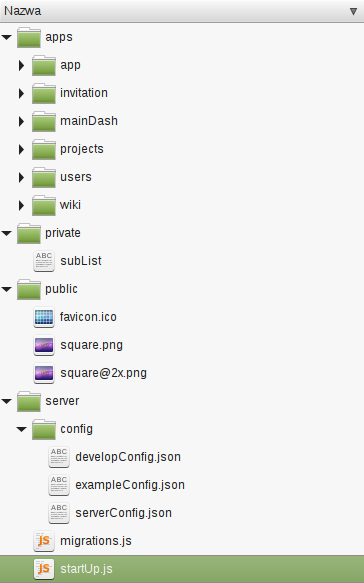
\includegraphics[width=0.5\textwidth]{ch03/intranet_005.png}
  \caption{Główny katalog aplikacji \emph{Intranet}}
  \label{fig:app_main_structure}
\end{figure}

Rysunek \ref{fig:app_main_structure} przedstawia główny katalog aplikacji \emph{Intranet}. Skład się on z następujących podkatalogów: \verb|apps|, \verb|private|, \verb|public|, \verb|server|. W katalogu \verb|apps| znajdują się poszczególne moduły aplikacji. Katalog \verb|private| zawiera zasoby nie dostępne z zewnątrz, znajduje się w nim opis subskrypcji wykorzystywanych przez aplikację. Katalog \verb|public| zawiera pliki graficzne używane przez aplikację. W katalogu \verb|server| znajduje się plik odpowiedzialny za migrację \verb|migrations.js| oraz plik \verb|startUp.js| zawierający kod uruchamiany na samym początku startu strony serwerowej. W podkatalogu \verb|config| zanajdują się pliki konfiguracyjne zapisane w postaci JSON. Plik \verb|developConfig.json| używany jest podczas pracy rozwojowych nad aplikacją. Plik \verb|serverConfig.json| używany jest w środowisku produkcyjnym.

Katalog \verb|apps| zawiera poszczególne moduły aplikacji. Podkatalog \verb|app| zawiera kod wykorzystywany w całej aplikacji, konfigurację używanych pluginów, globalne definicje \textit{helperów} --- funkcji pomocniczych używanych w szablonach HTML, pliki CSS wspólne dla całej aplikacji, pomocnicze szablony HTML oraz rozszerzenie wbudowanego obiektu szablonu o nową właściwość \verb|parentTemplate|.

\begin{figure}[h]
%   \centering
\dirtree{%
.1 intranet.
.2 apps.
.3 projects.
.4 client.
.5 addProjectForm.html.      
.5 addTalk.html.             
.5 addTalk.js.               
.5 projectAddUserForm.html.  
.5 projectAddUserForm.js.    
.5 projectTalks.js.
.5 projectMain.html.   
.5 projectMain.js.  
.5 projectRoutes.js. 
.5 projectTalks.html.
.5 styles.
.6 projet.less.
.5 talkElement.html.
.5 talkElement.js.
.4 lib.
.5 forms.js.  
.5 project.js.  
.5 projectsMethodes.js.  
.5 talks.js.
.4 server.
.5 projectPub.js.
.5 talksPub.js.
}
%     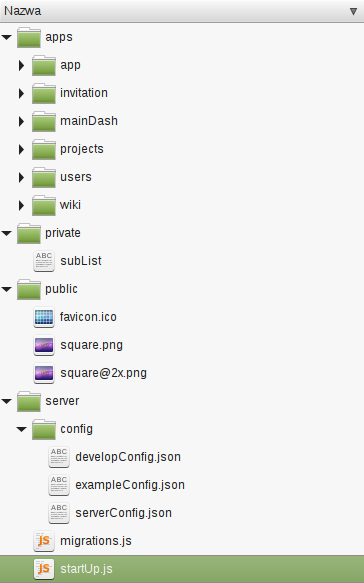
\includegraphics[width=0.5\textwidth]{ch03/intranet_005.png}
  \caption{Struktura przykładowego modułu \emph{projects}}
  \label{fig:app_project_structure}
\end{figure}

Rysunek \ref{fig:app_project_structure} przedstawia strukturę modułu \emph{projects} --- projekty. Widać w niej charakterystyczny podział aplikacji Meteor.js z wykorzystaniem katalogów specjalnych \verb|client| oraz \verb|server|. Katalog \verb|lib| zawiera kod wykorzystywany zarówno po stronie serwera jaki i klienta. Pliki zawarte w tym katalogu muszą zostać załadowane wcześniej niż kod znajdujący się w katalogach specjalnych. Kod ten zawiera definicje kolekcji projekty -- \verb|project.js| i konwersacji -- \verb|talks.js|, metody odpowiedzialne za operacje na danych w kolekcjach -- \verb|projectsMethodes.js| oraz definicje używanych przez moduł formularzy -- \verb|forms.js|. W katalogu \verb|client| znajdują się poszczególne widoki używane przez moduł oraz szablony poszczególnych elementów włączane przez inne szablony podczas renderowania ich zawartości. W pliku \verb|projectRoutes.js| zdefiniowane są trasy --- \textit{routing} --- dla modułu. Strona serwerowa składa się z dwu plików, które zawierają publikacje dla kolekcji jakich dostarcza moduł. Publikacje mogą być używane także poza modułem, w którym zostały zdefiniowane. Podkatalog \verb|styles| katalogu \verb|client| zawiera plik dynamicznego arkusza stylów less -- \verb|project.less|.

\section{Wspólna część dla strony serwerowej oraz klienckiej}

\subsection{Kolekcje} 
Dane, w bazie danych, wykorzystywane przez aplikację przechowane są w postaci dokumentów te natomiast grupowe są w logiczne zbiory nazywane kolekcjami. Klient oraz serwer używają tego samego API do dostępu do bazy danych. Klasa \verb|Mongo.Collection| używana jest do definiowania oraz manipulowania kolekcjami. Listing \ref{lst:project_coll} przedstawia sposób definicji kolekcji dla projektów --- \verb|Project|. Definicja jest umieszczona w katalogu \verb|lib| modułu \verb|projects|, który ładowany jest po stronie klienta jak i serwera przed plikami znajdującymi się w katalogach \verb|client| oraz \verb|server|. Tak zdefiniowaną kolekcję możemy używać po stronie serwera jak i klienta. 
\begin{js}[caption={{Definicja kolekcji dla projektów \textit{Project}}},label={lst:project_coll}]
Project = new Meteor.Collection('project');
\end{js}

Wykorzystując dodatkowy pakiet \verb|collection-hooks|\footnote{https://github.com/matb33/meteor-collection-hooks} możemy rozszerzyć klasę \linebreak \verb|Mongo.Collection| o dodatkowe właściwości dla operacji dodawania, modyfikowania oraz usuwania dokumentów w kolekcji wykonywane przed --- \verb|before| oraz po --- \verb|after| wykonaniu tych operacji. Przykładowe zastosowanie przedstawia listing \ref{lst:project_coll_hooks}. Rozszerzeniu ulegają operacje dodawania oraz modyfikacji. Przed wykonaniem operacji dodawania (\verb|insert|) dokumentu do kolekcji dodawane jest pole \verb|createdAt| z wartością ustawianą na dzisiejszą datę. Przed wykonywaniem operacji aktualizacji (\verb|update|) do modyfikatora jaki zostanie użyty podczas operacji aktualizacji dokumentu dodawane są pola \verb|modifiedAt| z wartością ustawioną na dzisiejszą datę oraz pole \verb|modifiedBy| z wartością jednoznacznie identyfikującą dokument użytkownika tak zwane \verb|_id| dokumentu.
Linia 12 listingu \ref{lst:project_coll_hooks} przedstawia użycie operatora \textit{lub} -- \verb|||| -- do przypisywania zmiennym, w tym przypadku argumentowi funkcji, wartości. Jeżeli argument ma wartość jego wartość się nie zmienia --- ulega ponownemu przypisaniu. Jeżeli natomiast wartość argumentu jest niezdefiniowana (\verb|undefined|) argumentowi przypisany zostanie pusty obiekt --- wyrażenie \verb|{}| jest literałem nowego obiektu. 
\begin{js}[caption={{Rozszerzanie kolekcji \textit{Project} o dodatkowe właściwości}},label={lst:project_coll_hooks}]
Project.before.insert(function (userId, doc) {
    "use strict";
    
    let createDate = new Date();
    doc.createdAt = createDate;
});

Project.before.update(function (userId, doc, fieldNames, modifier, options) {
    "use strict";
    
    let modDate = new Date();
    modifier.$set = modifier.$set || {};
    modifier.$set.modifiedAt = modDate;
    modifier.$set.modifiedBy = userId
});
\end{js}

\subsection{Metody}
Meteor.js oferuje mechanizm zdalnie wywoływanych metod. Klient może wywołać zdefiniowane metody zdalnie na serwerze. Metody są definiowane przez wywołanie \verb|Meteor.methodes|. Wywołanie \verb|Meteor.methodes| po stornie serwera tworzy funkcje, które mogą zostać zdalnie wywoływane przez klienta. Funkcje takie powinny zwracać wartość, która może zostać sparsowana do obiektu \textit{EJSON} lub zwracać błąd. Natomiast wywołanie \verb|methods| po stornie klienta definiuje funkcje typu \textit{stub} --- funkcja symulująca zachowanie metody o takiej samej nazwie  zdefiniowanej na serwerze. Jeżeli \textit{stub} zostanie zdefiniowany a klient wywoła metodę z nim powiązaną \textit{stub} zostanie wywołany równolegle. Po stronie klienta wartość zwracana przez \textit{stub} jest ignorowana. Funkcje \verb|stub| są uruchamiane dla ich skutków ubocznych --- ich celem jest symulacja wyników funkcji wywoływanych na serwerze bez konieczności oczekiwania na ich ukończenie oraz przesłanie ich wyniku z serwera.

\begin{js}[caption={{Wywołanie \textit{Meteor.methodes} oraz definiowanie metod}},label={lst:projects_methodes}]
Meteor.methods({
    removeUserFromProject (data) {
        check(data, {
            userId: String,
            projectId: String
        });
        
        let project = Project.findOne(data.projectId);
        if (Meteor.isServer) {
            
            if (!project || (!_.includes(project.secure.allowedUsers, this.userId) && project.secure.admin.id !== this.userId) ) {
                console.log('cant delete');
                throw new Meteor.Error(403, "Can't remove user from project");
            }
            Project.update({_id: project._id}, {$pull :{"secure.allowedUsers": data.userId, allowedUsers: data.userId}});
            return true;
        }


    },
    ...$
})

\end{js}
Wykorzystując \verb|Meteor.isServer| oraz \verb|Meteor.isClient| możemy rozdzielić kod metod na część wykonywaną tylko na serwerze, kliencie lub wspólnie dla obu przypadków. Definiując metody w części wspólnej dla serwera oraz klienta z wykorzystaniem powyższych elementów API możemy pominąć definiowanie \textit{stubów} dla metod po stronie klienta. Listing \ref{lst:projects_methodes} przedstawia  tak zdefiniowaną metodę umieszczoną w  pliku \verb|projectsMethodes.js| znajdującym się w katalogu \verb|lib|. Metody mogą przyjmować argumenty. Do sprawdzenia poprawność argumentów metody można skorzystać z funkcji sprawdzających wzorce takich jak \verb|check| oraz \verb|Match.test|. Funkcje te dostarczane są przez pakiet \verb|check|. Listing przedstawia usuwanie użytkownika z projektu. Linia 15 przedstawia aktualizację dokumentu w kolekcji \verb|Project| o podanym \verb|_id|. Z tablicy \verb|allowedUsers| usuwany jest ciąg znaków zawierających id danego użytkownika przekazane do metody w argumencie \verb|data|. Pierwszym atrybutem przejmowanym przez metodę \verb|update| wykonywaną na rzecz kolekcji to selektor określający jaki dokument lub dokumenty mają zostać zmodyfikowane. Drugi argument to modyfikator określający sposób modyfikacji danego dokumentu. 

\section{Serwer}
  \subsection{Baza}
  \subsection{Kolekcje}
  \subsubsection{Dostęp}
   allow/deny
   \subsubsection{Metody}
   \subsubsection{Publikacje}
% \subsection{Publikacje}
  \subsection{Migracje danych}
  \subsection{Konfiguracja}



\section{Klient}
  \subsection{Routing}
  \subsection{Subskrypcje}
  \subsection{Szablony}
    \subsubsection{HTML}
    \subsubsection{JS}
  \subsection{Eventy}
  \subsection{Helpery}
  \subsection{Pliki less}
    że są zbierane w całość i łączone w jeden duży plik.
  \subsection{Formularze}
    opis jak to jest obsługiwane plus yfform
  
\section{Objekt MyApp}
  po co go się stosuje

  
\section{Paczki powtstałe na potrzeby aplikacji}
yp2:admin-lte@2.3.1
yp2:confirm-modal-bs3@1.1.1
yp2:hijack-email@1.0.0
yp2:yfform@0.3.10
plus informacje że są one dostępne na Atmosfer i githubie